\documentclass[../main.tex]{subfiles}
\graphicspath{{img/}}
\begin{document}



\section{Triggerless DAQs}

\begin{comment}
importanza di triggerless o streaming readout DAQs in modern physics.
Una sempre più vasta quantità di dati viene prodotta dai moderni esperimenti di fisica ad alte energie,
\end{comment}

I moderni esperimenti nell'ambito della fisica ad alte energie producono sempre più vaste quantità di dati le quali devono essere selezionate, aggregate e salvate in memoria per poter essere analizzate.  
Per questo, si realizzano dei meccanismi di selezione dei dati (trigger) in base alle necessità dell'esperimento e al fenomeno fisico di interesse. Questo permette di ridurre il flusso di dati di diversi ordini di grandezza. L'evoluzione delle capacità di calcolo dei computer permette oggi di sostituire i classici trigger basati su circuiti elettronici con implementazioni software in grado di tenere conto di maggiori informazioni e selezionare i dati in modo più completo ed efficiente.  
Un sistema di questo tipo è stato sviluppato nell'ambito del progetto NEMO (NEutrino Mediterranean Observatory) per eseguire il filtraggio e l'acquisizione dei dati. L'esperimento prevede rivelatori a scintillazione ancorati al fondale marino, tramite i quali rivelare la radiazione cherenkov emessa dalle particelle cariche generate dalla collisione tra neutrini cosmici e il fondale marino o le molecole d'acqua. La locazione sottomarina dell'esperimento ha richiesto la semplificazione dell'hardware dei rilevatori. Quindi tutti i dati sono inviati a terra dove TriDAS (Triggerless Data Acquisition System) realizza la selezione e l'archiviazione dei dati.
TriDAS è stato scritto in modo da essere scalabile e adattabile flessibile a diverse configurazioni di rilevatori. Infatti il progetto NEMO stava verificando le condizioni di realizzazione dell'esperimento europeo KM3Net che prevedeva un maggior numero di rilevatori in configurazioni diverse. Questo ha reso TriDAS capace di gestire esperimenti in ambiti diversi come gli esperimenti di collisione di fascio ai Jefferson Lab (Newport, Virginia).




\section{TriDAS-core}


\begin{figure}[tb]
    \centering
    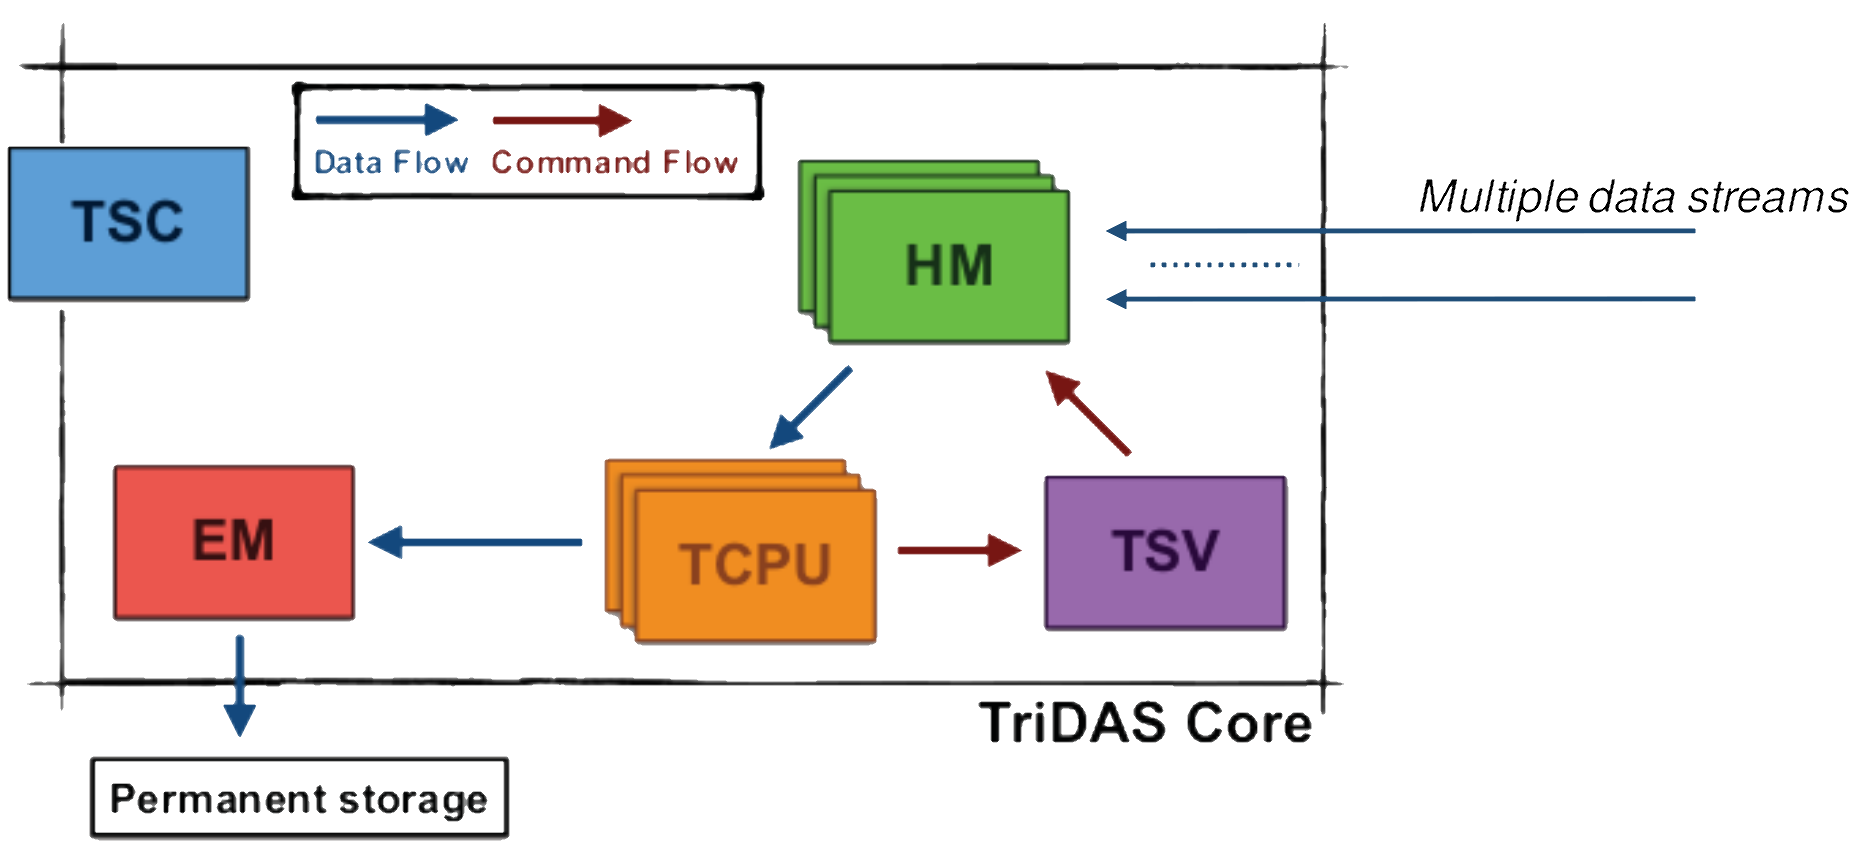
\includegraphics[width=\textwidth]{tridas_scheme_more_trasp.png}
    \caption{
	    Rappresentazione dei componenti di TriDAS e delle loro interazioni. Flussi continui di dati provenienti dall'elettronica dell'esperimento vengono inviati agli \emph{Hit Managers} (HMs) i quali li dividono in pacchetti di lunghezza prefissata. Condividendo lo stesso orologio, gli HM inviano a una \emph{Trigger CPU} (TCPU) i pacchetti dei diversi flussi di dati che si riferiscono allo stesso intervallo di tempo. Il \emph{TriDAS Supervisor} (TSV) regola questo scambio indicando agli HMs quale TCPU sia disponibile a processare i dati. Quindi, la TCPU sottopone i dati agli algoritmi di trigger e invia all'\emph{Event Manager} (EM) le porzioni di segnale che li hanno soddisfatti, per essere salvati in memoria. L'utente interagisce e configura il sistema tramite il \emph{TriDAS System Controller} (TSC).  
	\cite{chiarusi}}
    \label{fig:tridas}
\end{figure}

\begin{figure}[tb]
    \centering
    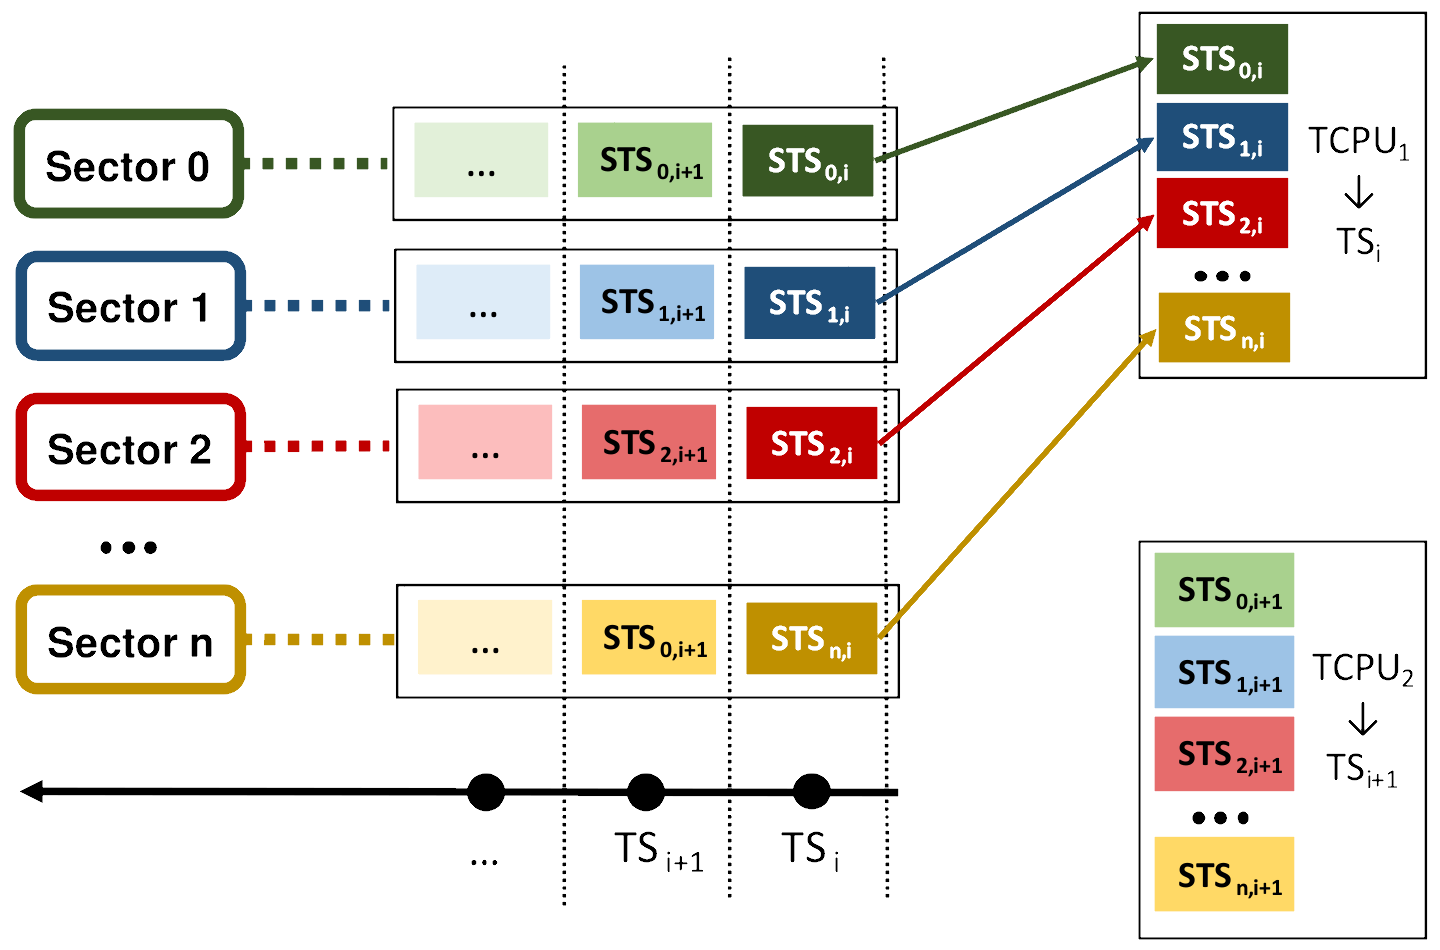
\includegraphics[width=\textwidth]{hm_trasp.png}
    \caption{L'esperimento ideato da Rutherford prevede un bersaglio d'oro di appena \SI{8.6e-6}{\cm} di spessore, irradiato da un flusso di particelle $\alpha$ generate dal decadimento di una lastra di radon. Il bersaglio è circondato da vetro dipinto con solfuro di zinco (ZnS), che scintilla al contatto con particelle cariche. Le particelle $\alpha$, cariche positivamente, in alcuni casi proseguono indisturbate e in altri vengono deviate a grandi angoli, fino anche ad essere respinte. Ciò dimostra l'inesattezza del modello atomico di Thomson, in cui la carica positiva dell'atomo ne riempie tutto il volume. Invece deve esistere all'interno dell'atomo una concentrazione di carica positiva abbastanza alta da poter deviare le pesanti particelle $\alpha$. \cite{chiarusi}}
    \label{fig:hmtcpu}
\end{figure}


\begin{figure}[tb]
    \centering
    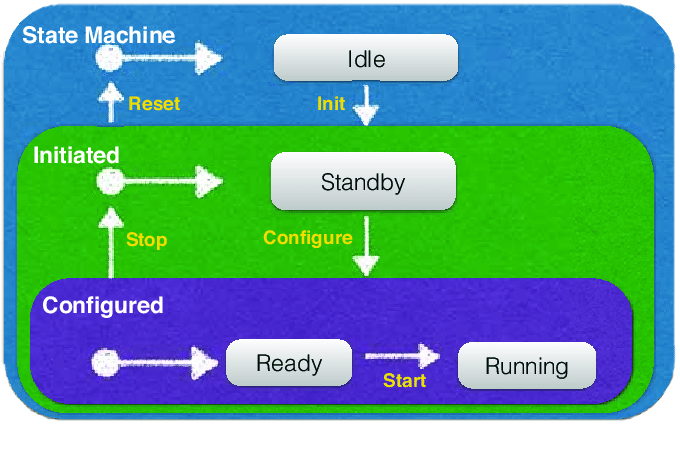
\includegraphics[width=0.5\textwidth]{tsc_scheme_color_better.png}
    \caption{L'esperimento ideato da Rutherford prevede un bersaglio d'oro di appena \SI{8.6e-6}{\cm} di spessore, irradiato da un flusso di particelle $\alpha$ generate dal decadimento di una lastra di radon. Il bersaglio è circondato da vetro dipinto con solfuro di zinco (ZnS), che scintilla al contatto con particelle cariche. Le particelle $\alpha$, cariche positivamente, in alcuni casi proseguono indisturbate e in altri vengono deviate a grandi angoli, fino anche ad essere respinte. Ciò dimostra l'inesattezza del modello atomico di Thomson, in cui la carica positiva dell'atomo ne riempie tutto il volume. Invece deve esistere all'interno dell'atomo una concentrazione di carica positiva abbastanza alta da poter deviare le pesanti particelle $\alpha$. \cite{chiarusi}}
    \label{fig:tsc}
\end{figure}

TriDAS (Triggerless Data Acquisition System) è un sistema di acquisizione dati \emph{triggerless} sviluppato originariamente per il prototipo di rilevatore per neutrini \mbox{NEMO}. NEMO aveva come scopo verificare e realizzare le tecnologie per realizzare il rilevatore sottomarino KM3Net, i cui sensori sono distribuiti su un volume di un kilometro cubo, e per questo ha avuto uno sviluppo graduale secondo diverse fasi di test. Quindi, uno dei requisiti di TriDAS era essere scalabile con l'evoluzione della struttura del rilevatore. Per questo, TriDAS implementa un design modulare, che gli ha permesso di essere adattato a un esperimento di collisione di fascio di particelle con facilità.

TriDAS è costituito da vari componenti software scritti in \texttt{C++11}, ciascuno con un ruolo specifico nella catena di elaborazione e acquisizione dati (fig. \ref{fig:tridas}).
Gli \emph{HitManager}s (HMs) sono il primo punto di aggregazione dei dati. 
Ciascun \textbf{settore} del rilevatore (tipicamente un gruppo di sensori), invia un flusso continuo di dati a un HM. L'HM quindi divide il flusso di dati in buffer ordinati temporalmente di durata definita dall'utente detti \emph{Sector Time Slice} (STS). Essendo sincronizzati temporalmente, gli HMs inviano a una TCPU tutte le STS che si riferiscono allo stesso intervallo di tempo, detto \emph{Time Slice} (TS) (fig. \ref{fig:hmtcpu}).  
Il \emph{TriDAS Supervisor}
La \emph{Trigger CPU} (TCPU) quindi organizza tutte le STS ricevute in un oggetto unico detto \emph{Telescope Time Slice} e lo sottopone agli algoritmi di trigger. Un livello iniziale di trigger detto \emph{L1} implementa come criterio una soglia di ampiezza di segnale definita dall'utente. Livelli successivi  di trigger possono essere definiti e attivati dall'utente. Ciascun algoritmo di trigger viene eseguito su un \emph{thread} differente, che viene fatto partire all'avvio della TCPU, dopo aver caricato dinamicamente la corrispondente libreria.  Quindi diversi algoritmi di trigger possono essere eseguiti contemporaneamente in una TCPU sulla stessa TTS. Ogni volta che una condizione di trigger è soddisfatta, un sottoinsieme dei dati chiamato \emph{Triggered Event} (TE) comprendente un intervallo di segnale centrato nel seed del trigger di ampiezza variabile (tipicamente \SI{6}{\ns}) viene inviato all'\emph{Event Manager}. 
L'\emph{Event Manager} (EM) aggrega i TE di ciascun algoritmo, verifica possibili duplicati, e li scrive su disco in un file formato \emph{Post Trigger} (PT).




\section{detector setup at Jefferson Lab}

\end{document}
